\chapter{网络流}

\begin{introduction}
	\item 网络流
	\item 最大流
	\item Ford-Fulkerson算法
	\item 残差图与增广路径
\end{introduction}

\section{网络流}

\subsection{什么是网络流}

	\par 简单地说,网络流是图上的一种映射关系,但也可以理解为一个图生成的一个有向子图,且这个子图受到图本身条件的限制。
		形象地说,就好比一个管道网络和其中流淌的水。下面给出网络流的形式化描述。

\begin{definition}{网络流定义}{network-flow}
	对有向图\(G(V, E)\),
	图中有源点\(s\)和汇点\(t\),且\(s, t \in V,\ s \ne t\),
	\(E\)中边的容量\(C\)是一个映射\(C:E \to N\ or\ R^+\)。
	定义流(flow)是\((G, C)\)上的一个映射\(f:E \to N\ or\ R^+\),满足下列约束:
	
	\begin{enumerate}[(1)]
	\item 容量限制:对\(\forall\ e \in E,\ f(e) \le C(e)\);
	
	\item 流量守恒:对\(\forall\ v \in V / \{s, t\},\ f_{in}(v) = f_{out}(v)\),
	其中
	\begin{equation}\nonumber
	f_{in}(v) = \sum_{(u,v) \in E, u \in V} f(u,v)
	\end{equation}
	\begin{equation}\nonumber
	f_{out}(v) = \sum_{(v,u) \in E, u \in V} f(v,u)
	\end{equation}
	
	特别地,\(s\)的入度、\(t\)的出度为0。
	\end{enumerate}

\end{definition}

	\par 对于一个网络流,我们通常使用流的价值(大小)来进行评价。流的价值描述如下。

\begin{definition}{流的价值}{value-of-a-flow}
	一个网络流\(f\)的价值记为\(|f|\),有
	
	\begin{equation}
	|f| = \sum_{(s,v) \in E, v \in V} f(s,v) = \sum_{(v,t) \in E, v \in V} f(v,t)
	\end{equation}
	
	也就是源点\(s\)的出度、汇点\(t\)的入度。
	
\end{definition}

\subsection{网络流的\(s-t\)割}

	\par 为了辅助分析网络流,引入\(s-t\)割的概念。

\begin{definition}{\(s-t\)割}{s-t-cut}
	一个\(s-t\)割是对点的一种划分,记为\(cut(A, B)\),将图\(G\)的点集\(V\)划分成\(A, B\)两部分,使得
	\(A \cup B = V,\ A \cap B = \varnothing,\ s \in A,\ t \in B\)。
\end{definition}

	\par 注意,这与通常所说的割集有所不同。\(s-t\)割是一种划分方式,而割集是边的集合。
	对一个连通图而言,去掉一个割集中的所有边,将使得这个图不再连通,分为\(A,\ B\)两个连通子图;但若少去掉其中的任何一条,它仍然还是连通的。

\begin{proposition}{\(s-t\)割的性质}{s-t-cut-prop}
	对\(\forall f\), \(\forall cut(A, B)\)有
	\begin{equation}
		f(A,B) \triangleq \sum_{u \in A, v \in B, (u,v) \in E} f(u,v) - \sum_{u \in A, v \in B, (v,u) \in E} f(v,u) = |f|
	\end{equation}
\end{proposition}

\begin{proof}
	通过归纳法证明。
	\begin{enumerate}[(1)]
	\item 若\(|A| = 1\),即\(A = \{s\},\ B = V / \{s\}\),有\(f(A, B) = f_{out}(s) = |f|\);
	\item 向\(A\)中添加相邻点\(v\),则
	\begin{equation}\nonumber
		f(A, B) = f_{out}(s) + f_{out}(v) - f_{in}(v)
	\end{equation}
	由流量守恒可知
	\begin{equation}\nonumber
		f_{in}(v) = f_{out}(v)
	\end{equation}
	因此仍有\(f(A, B) = |f|\);
	\item 重复以上归纳直至\(A = V / \{t\},\ B = \{t\}\)。
	\end{enumerate}
\end{proof}

\begin{definition}{\(s-t\)割的容量}{s-t-cut-capacity}
	一个\(s-t\)割\(cut(A, B)\)的容量记为\(C(A, B)\),有
	\begin{equation}
		C(A,B) = \sum_{u \in A, v \in B, (u,v) \in E} C(u,v)
	\end{equation}
\end{definition}

\begin{proposition}{\(s-t\)割容量的性质}{s-t-cut-capacity-prop}
	给定任一\(s-t\)割\(cut(A, B)\),对\(\forall f\)有
	\begin{equation}
		f(A,B) \le C(A, B)
	\end{equation}
\end{proposition}

\begin{proof}
	\begin{equation}\nonumber
		\begin{split}
		f(A,B)& = \sum_{u \in A, v \in B, (u,v) \in E} f(u,v) - \sum_{u \in A, v \in B, (v,u) \in E} f(v,u) \\
			& \le \sum_{u \in A, v \in B, (u,v) \in E} f(u,v) \\
			& \le \sum_{u \in A, v \in B, (u,v) \in E} C(u,v) = C(A,B)
		\end{split}
	\end{equation}
\end{proof}


\section{最大流与Ford-Fulkerson算法}

	\par 对于网络流问题,我们通常关注的是流的价值,并总是希望找到价值最大的流。
	这在很多应用场景中都有可能涉及到,而且对于很多其他类型的问题,都可以转化成网络流问题来求解。
	在一个图中求解最大流的问题,称为最大流问题。

\begin{definition}{最大流}{max-flow}
	在一个有向图\(G(V, E)\)中,最大流\(f_{max}\)为价值最大的流,即\(f_{max} = arg\ max\ |f|\)。
\end{definition}

\subsection{贪心策略}

	\par 在一个有向图\(G(V, E)\)上,可以有很多个流,如何求得其中的最大流呢?
	我们首先可以尝试使用贪心的思路求解,尽可能地从源点\(s\)向汇点\(t\)输送更多的流。
	所谓流的输送,就是找到一条从\(s\)到\(t\)的路径,在该路径上建立流的映射关系。
	由于一个流需要满足容量限制和流量守恒的约束,因此在此引入瓶颈容量的概念。

\begin{definition}{瓶颈容量}{bottle-neck-capacity}
	在图的一条路径中,该路径上容量最小的边的容量称为瓶颈容量。
\end{definition}

	\par 当在一条路径上输送流量时,最多输送的流的大小只能是瓶颈容量的值。
	另外,当一条边上有流量通过时,该边的容量也就少了该边上的流值。
	求解最大流问题时,有向图边的容量即为边的权值,当边的容量为0时,视为去掉该边,变为不连通。

	下面给出一个贪心策略。

\begin{algorithm}
	\caption{求最大流的贪心尝试}\label{alg:greedy-max-flow}
	\KwIn{图$G$,源点$s$,汇点$t$}
	\KwData{流的值$f$ = 0}
	\Begin{
		\While{$G$中存在$s$到$t$的路径}{
			选择其中瓶颈容量最大的路径\\
			在该路径上输送其瓶颈容量大小的流量,并更新路径上各边的剩余容量值\\
			$f$增加该路径瓶颈容量值的大小
		}
	}
	\Return{$f$}
\end{algorithm}

	\par 这个贪心算法看起来很简单,那么其正确性如何呢?当然没这么容易。下例是一个简单反例。

\begin{example}
	用上述贪心策略求出下图中的最大流。

	\begin{figure}[hbt]
		\centering
		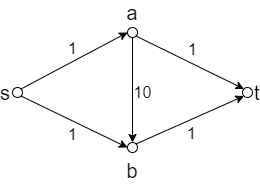
\includegraphics[scale=0.5]{image/network-flow-greedy-example.png}
		\caption{一个网络流算例}
	\end{figure}\label{fig:max-flow-greedy-fig1}
	\par 容易看出这个例子的最大流为2,即通过\(s \to a \to t\)和\(s \to b \to t\)两条路径各输送1个流量。
	但上述贪心算法不能保证这个结果,因为它第一次找到的路径可能是\(s \to a \to b \to t\),则输送流量后,
	剩余容量更新为以下形式。

	\begin{figure}[hbt]
		\centering
		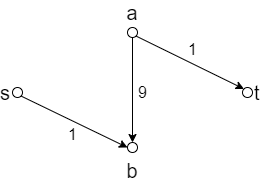
\includegraphics[scale=0.5]{image/network-flow-greedy-example2.png}
		\caption{通过路径\(s \to a \to b \to t\)输送1个流量后的容量剩余情况}\label{fig:max-flow-greedy-fig2}
	\end{figure}
	\par 此时,图中不再有\(s \to t\)的路径,贪心算法结束,但求得的结果不是最大流。

\end{example}

	\par 尝试更换另一种贪心策略,如最短路径优先,可不可行呢?
	只需将\autoref{fig:max-flow-greedy-fig1}中的图修改为以下形式,
	在\autoref{fig:max-flow-greedy-fig3}中,\(s\)到\(b\)和\(a\)到\(t\)之间各有十个以上的点依次相连,各边容量都大于等于1,
	易知最大流的值也是2。
	但此时,贪心算法仍会选择路径\(s \to a \to b \to t\),因为它最短,从而得到同样的错误结果。

	\begin{figure}[hbt]
		\centering
		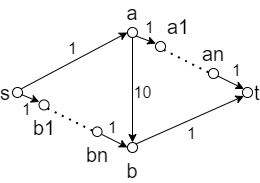
\includegraphics[scale=0.5]{image/network-flow-greedy-example3.png}
		\caption{最短路径优先的贪心策略的反例}\label{fig:max-flow-greedy-fig3}
	\end{figure}

	\par 简单的贪心策略似乎不能有效求解最大流问题,那么正确的方法是什么呢?

\subsection{Ford-Fulkerson算法}

	\par Ford-Fulkerson算法于1956年提出,简称FF算法,直到现在仍是许多现代最大流求解算法的基础。
	严格地说,FF算法并不是“算法”,而是一种方法,因为其中的一些操作是不确定的,需要实现者自行选择策略。
	
	\par FF算法的主要思想是允许反悔。也就是说,当流量经过了一条不合适的路径后,能够反悔,进行回溯。
	如何实现这一机制呢?如何保证反悔后不会重蹈覆辙?首先引入残差图的概念。

\begin{definition}{残差图}{residual-graph}
	残差图也是一个有向图。对给定的图\(G(V,E)\)和图上现有的一个流\(f\),构造对应的残差图,记为\(G_f\)。
	构造规则如下:
	\begin{enumerate}[(1)]
		\item 对\(G\)中的所有有流量的边\(e=(u,v),\ u,v\in V\),在残差图\(G_f\)中加入该边,
			其残差容量\(C_f(e)=C(e)-f(e)\)。
			同时,也向\(G_f\)中加入其反向边\(e'=(v,u)\),其中\(C_f(e')=f(e)\);
		\item 在残差图\(G_f\)上操作流量时,所有边都是可走的。在路径上输送流量时,同样更新路径上所有边的残差容量\(C_f\)。
			若对某一个边\(e\),它没有反向边,则按同样规则加入反向边,若已有反向边\(e'\),则使\(C_f(e')\)增加新流量的值;
		\item 当\(G_f\)中某一边的的残差容量减至0时,将其从\(G_f\)中去掉。
	\end{enumerate}
\end{definition}

	\par 由残差图的构造方式可知,当\(G\)中没有流量时,\(G_f\)与\(G\)是相同的。对\autoref{fig:max-flow-greedy-fig2}中的情况,
		给出对应的残差图,如\autoref{fig:residual-graph1}所示。当在路径\(s \to a \to b \to t\)上输送一个流量后,
		\((s,a),\ (b,t)\)上的残差容量减为0,从残差图中去掉;\((a,b)\)上的残差容量减少1;同时为路径上的所有边更新了反向边。
	
		\begin{figure}[hbt]
			\centering
			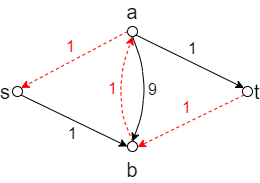
\includegraphics[scale=0.5]{image/network-flow-residual-graph1.png}
			\caption{通过路径\(s \to a \to b \to t\)输送1个流量后的残差图}\label{fig:residual-graph1}
		\end{figure}


	\par 在残差图的基础上,引入增广路径的概念。

\begin{definition}{增广路径}{argument-path}
	对给定的图\(G(V,E)\)和图上现有的一个流\(f\),一条增广路径是相应的残差图\(G_f\)上的一条从\(s\)到\(t\)的简单路径。
\end{definition}

	\par 引入残差图和增广路径的概念,通过添加反向边,提供了一种反悔回溯的方式,这就是FF算法的妙处。以下给出FF算法的描述。

\begin{algorithm}[hbt]
	\caption{Ford-Fulkerson算法}\label{alg:ford-fulkerson}
	\KwIn{图$G$}
	\KwData{流的值$f$ = 0}
	\Begin{
		由$G$得到残差图$G_f$\\
		\While{$G_f$中存在增广路径}{
			选择某一条增广路径输送流量,并更新路径上各边和反向边的残差容量\\
			$f$增加输送流量的大小
		}
	}
	\Return{$f$}
\end{algorithm}

	\par 对于\autoref{fig:residual-graph1}中的情形,FF算法还可在图中找到\(s \to b \to a \to t\)这样一条增广路径,
	相当于对先前走边\((a,b)\)进行了反悔,最终找到了最大流。

	\par 从FF算法的描述中可以注意到,其中确实存在不明确的操作,也就是未提及增广路径的选择策略。
	不同的选择策略可能会带来性能上差异,这里暂时不讨论。

	\par 有了FF算法,如何说明其正确性呢?通过以下引理,可以证明FF算法是正确的。

\begin{lemma}{}{max-flow-lemma1}
	对于给定的图\(G(V,E)\)和一个流\(f\),以下命题是等价的:
	\begin{enumerate}[(1)]
		\item \(f\)是最大流;
		\item \(G\)的残差图\(G_f\)中,不存在\(s \to t\)的路径,即增广路径。
	\end{enumerate}
\end{lemma}

\begin{proof}
	\begin{enumerate}[a)]
		\item (1) $\rightarrow$ (2):

			采用反证法,即证明$\neg$ (2) $\rightarrow$ $\neg$(1)。
			假设\(f\)是最大流,若\(G_f\)中仍存在增广路径,设其瓶颈容量为\(\Delta f\),
			则从\(s \to t\)还可以输送\(\Delta f\)的流量,即存在大小为\(f + \Delta f\)的流,使得
			\begin{equation}\nonumber
				f + \Delta f > f
			\end{equation}
			因此\(f\)不是最大流。
		\item (2) $\rightarrow$ (1):

			在残差图\(G_f\)中,将从源点\(s\)出发仍有路径可达的所有点以及源点\(s\)设为点集\(A\),图中的其他点构成点集\(B\)。
			因为\(G_f\)中不存在\(s \to t\)的路径,所以\(t \in B\),由定义\ref{def:s-t-cut}可知,这实际上构成了一个\(s-t\)割\(cut(A,B)\)。
			\begin{figure}[hbt]
				\centering
				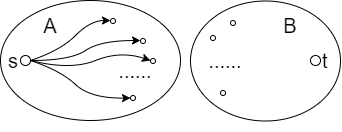
\includegraphics[scale=0.5]{image/network-flow-ff-proof-graph1.png}
				\caption{构造一个\(s-t\)割}\label{fig:ff-proof-graph1}
			\end{figure}

			在原图\(G\)中,由连通性的要求,一定存在点集\(A\)与点集\(B\)之间的边,这些边中有从\(A\)到\(B\)的,也可能有从\(B\)到\(A\)的,
			如\autoref{fig:ff-proof-graph2}所示。
			
			对于从\(A\)到\(B\)的边,如\((a_1,b_1)\),边上的流量\(f(a_1,b_1)\)一定是等于边的容量\(C(a_1,b_1)\)的,
			否则,在残差图\(G_f\)中,\((a_1,b_1)\)的残差容量\(C_f(a_1,b_1)\)就不为0,使得仍有从\(A\)到\(B\)的路径。
			
			对于从\(B\)到\(A\)的边,如\((b_n,a_3)\),边上的流量\(f(b_n,a_3)\)一定为0,
			否则,在残差图\(G_f\)中就会存在反向边\((a_3,b_n)\),且其残差容量为\(f(b_n,a_3)\)的值,也使得从\(A\)到\(B\)有路径。
			\begin{figure}[hbt]
				\centering
				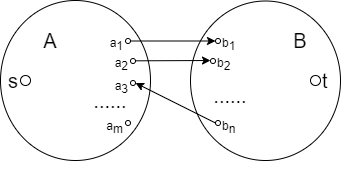
\includegraphics[scale=0.5]{image/network-flow-ff-proof-graph2.png}
				\caption{原图\(G\)上的\(cut(A,B)\)}\label{fig:ff-proof-graph2}
			\end{figure}

			基于上述观察,对于\(cut(A,B)\),有
			\begin{equation}\nonumber
				\begin{split}
				|f| = f(A, B)& = \sum_{u \in A, v \in B, (u,v) \in E} f(u,v) - \sum_{u \in A, v \in B, (v,u) \in E} f(v,u)\\
				& = \sum_{u \in A, v \in B, (u,v) \in E} f(u,v)\\
				& = C(A, B)
				\end{split}
			\end{equation}

			因为流\(f\)是不依赖于\(s-t\)割的,根据性质\ref{pro:s-t-cut-capacity-prop},对于一个图上任意的\(s-t\)割,流值总是小于其容量的,
			也就是说,任何流的值总小于等于容量最小的\(s-t\)割的容量。
			此时,流\(f\)的值等于\(C(A,B)\),表明\(cut(A,B)\)就是容量最小的\(s-t\)割,而\(f\)就是最大流。

	\end{enumerate}
\end{proof}

	\par 在FF算法中,算法会运行至残差图中没有增广路径为止,结束时求得的流就是最大流。以上证明也间接证明了其正确性。
	此外,由该证明过程可以导出一个定理,即最大流最小割定理。

\begin{theorem}{最大流最小割定理}{maximum-flow-minimum-cut-theorem}
	对于一个有向图\(G\),其最大流的值等于其容量最小的\(s-t\)割的容量值。
\end{theorem}

\subsection{Ford-Fulkerson算法的实现及其时间复杂度}
\par 基于DFS实现的FF算法是FF算法的最基础的实现形式,其算法描述如下

\begin{algorithm}
\caption{基于DFS的FF算法}\label{alg:ford-fulkerson}
\KwIn{图 $G$,其中$s$和$t$分别为其源点和汇点}
\KwData{流的值$f$ = 0}
\Begin{
	$tmp$ = dfs($G$, $s$, $inf$)

	\While{$tmp$ > 0}{
		$f$ = $f$ + $tmp$
	}
	\Return{$f$}
}

\end{algorithm}

\par 其中,dfs()算法通过深度优先的方式在图$G$中寻找增广路径,并返回所找到的增广路径的流量。同时,按照FF算法的要求,其在寻找增广路径的过程中会更新增广路径上各边的残差容量。其实现可以描述如下

\begin{algorithm}
\caption{dfs()}
\KwIn{图$G$,当前节点$p$,当前流值$flow$}
\KwData{流值$ret$}
\Begin{
	\If{$p$ = $t$} {
		\Return{$flow$}
	}
	\For{$next$为$p$的下一节点}{
		$tmp$ = dfs($G$,$p$,min($flow$,c($p$,$next$)))

		\If{$tmp$ > 0}{
			c($p$,$next$) = c($p$,$next$) - $tmp$	
	
			c($next$,$p$) = c($next$,$p$) + $tmp$

			\Return{$tmp$}
		}
	}
	\Return{0}
}
\end{algorithm}

\par 不难推算出,该算法的时间复杂度为$O(mf)$,其中$m$为图$G$中边的数量,$f$为最大流。同时,需要注意的是,该算法并不能有效的处理环的情况。当图中存在环的时候,该算法很有可能陷入无限的循环之中。当然,这可以通过众多的改进措施避免。

\par 然而,现在最常见的网络流算法是Dinic算法。其可以有效的避免因为图中存在环状结构而陷入死循环的问题。同时,因为采用了分层的机制,其时间复杂度也有所降低,为$O(m^2n)$。给出Dinic算法的伪代码描述如下。

\begin{algorithm}
\caption{Dinic()}
\KwIn{图$G$}
\KwData{最大流值$f$}
\Begin{
	$f$ = 0

	\While{bfs($G$) != 0}{
		$tmp$ = dfs($G$,$s$,$inf$)

		\If{$tmp$ <= 0} {
			\Return{$f$}
		}
		$f$ = $f$ + $tmp$
	}
}
\end{algorithm}

\par 其中,bfs()算法负责为当前的图按照广度优先的策略“分层”,并返回$t$点的层数。分层的主要目的是加速dfs()算法查找增广路径的速度,并避免算法陷入死循环之中。dfs()算法则与上文中提到的类似,但其每次迭代均只会选择层数高于当前节点的节点。下文给出bfs()算法的代码描述。而dfs()算法则可在上文dfs()算法的基础上进行简单修改得到。

\begin{algorithm}
\caption{bfs()}
\KwIn{图$G$,其中所有节点的层数均为0}
\KwData{节点$t$的层数}

\Begin{
	将$s$的层数设置为$level$

	将$s$压入栈$stack$中

	\While{$stack$不为空}{
		从$stack$中出栈节点$node$,其层数为$level$

		\For{$n$为$node$的子节点}{
			\If{$n$的层数为0}{
				将$n$的层数设置为$level$+1

				将$n$压入$stack$
			}
		}
	}

	\Return{$t$的层数}
}
\end{algorithm}

\par 当然,除了上述的两种FF算法的实现外,还有众多算法可以实现FF算法所描述的思想。诸如WAP(Widest Argumentary Path)算法、SAP(Shortest Argumentary Path)算法等。这些算法着眼于优化FF算法中寻找增广路径的部分,并且较之基本的FF算法有着更优的时间复杂度。限于篇幅此处不一一赘述,感兴趣的读者可以自行去查找相关资料。

\subsection{FF算法的局限性}

\par 我们可以看到,FF算法能够很好地解决边权为有理数的图的最大流问题,但其无法很好地解决边权为无理数的图的最大流问题。我们可以通过一个例子来解释这个问题。假设有$r^2=1-r$,考虑下图的情况

\begin{figure}[hbt]
	\centering
	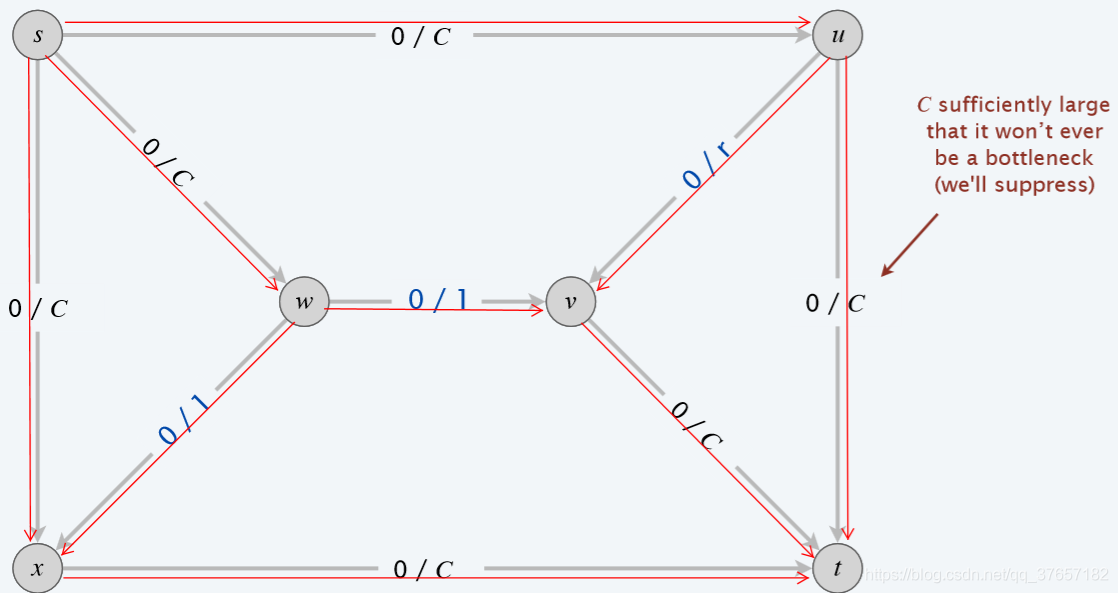
\includegraphics[scale=0.4]{image/network-flow-backbone1.png}
	\caption{Ford-Fulkerson算法的缺陷(1)}\label{fig:network-flow-backbone1}
\end{figure}

\begin{figure}[hbt]
	\centering
	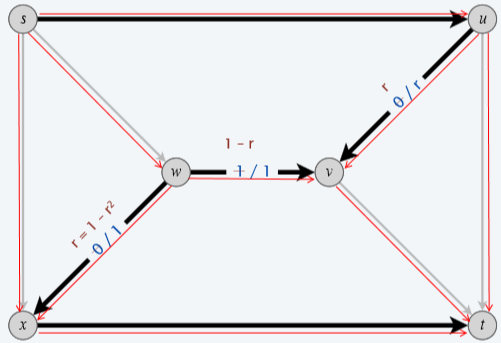
\includegraphics[scale=0.6]{image/network-flow-backbone2.png}
	\caption{Ford-Fulkerson算法的缺陷(2)}\label{fig:network-flow-backbone2}
\end{figure}

\begin{figure}[hbt]
	\centering
	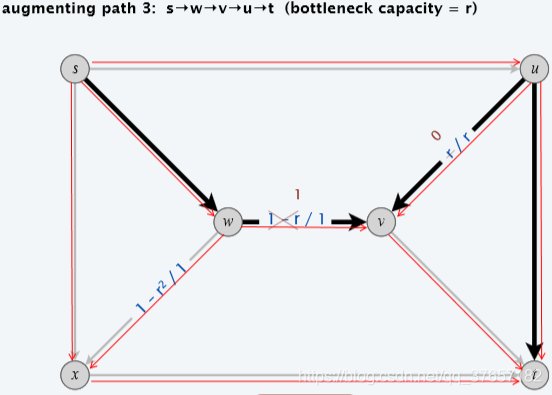
\includegraphics[scale=0.6]{image/network-flow-backbone3.png}
	\caption{Ford-Fulkerson算法的缺陷(3)}\label{fig:network-flow-backbone3}
\end{figure}

\begin{figure}[hbt]
	\centering
	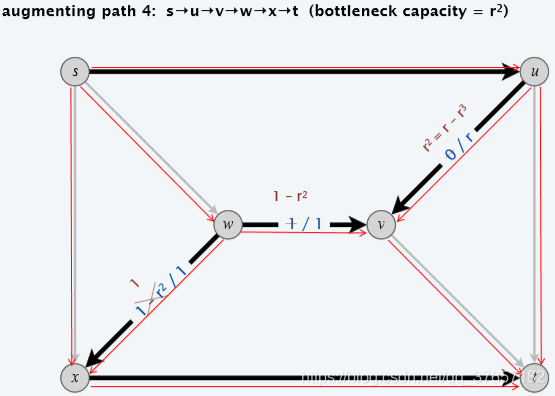
\includegraphics[scale=0.6]{image/network-flow-backbone4.png}
	\caption{Ford-Fulkerson算法的缺陷(4)}\label{fig:network-flow-backbone4}
\end{figure}

\begin{figure}[hbt]
	\centering
	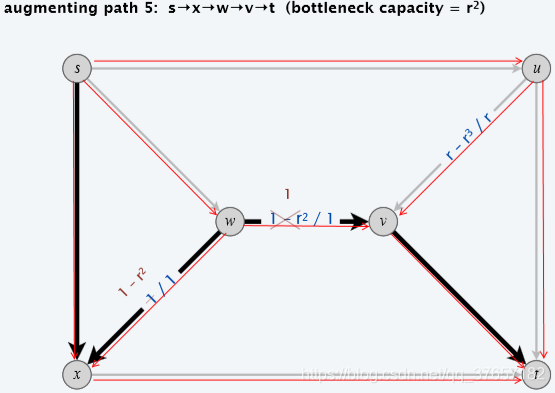
\includegraphics[scale=0.6]{image/network-flow-backbone5.png}
	\caption{Ford-Fulkerson算法的缺陷(5)}\label{fig:network-flow-backbone5}
\end{figure}

\begin{figure}[hbt]
	\centering
	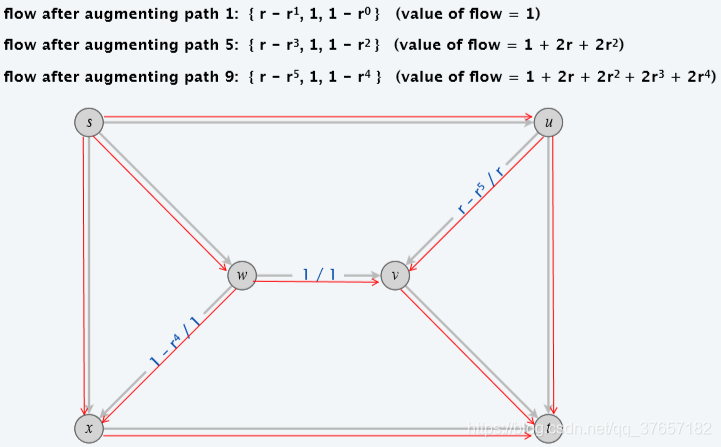
\includegraphics[scale=0.6]{image/network-flow-backbone6.png}
	\caption{Ford-Fulkerson算法的缺陷(6)}\label{fig:network-flow-backbone6}
\end{figure}

\par 可以看见,FF算法并不会停下来。相反的,因为各边边权的这种奇妙的关系,算法会无休止地运行下去。其所得到的流值最终仍会收敛,但却会收敛到一个错误的值上。从这个例子可以看到,FF并不适合于某些边权为无理数的图。